\begin{itemize}
\item Sources/loads
\item If we know all the information about the source, we can calculate the power drawn by any load
  \begin{itemize}
  \item Use voltage division to find voltage $V_0 = V_s \frac{R_0}{R_s+R_0}$
  \item $P_0=V_0^2/R_0$
  \end{itemize}
\item When we ask the question ``What load will draw the maximum power?'', we need to dip into Calculus
  \begin{itemize}
  \item The maximum of a function $f(x)$ occurs when the derivative $f'(x)$ goes to zero
  \item Our function is $\displaystyle P_0(R_0)=\left( V_s \frac{R_0}{R_s+R_0}\right)^2 \cdot \frac{1}{R_0}$
  \item We need to solve $\displaystyle P_0'(R_0) = V_s^2 \cdot \frac{(R_s^2+R_0^2)-R_0\cdot 2 R_0}{(R_s^2+R_0^2)^2} = 0$
  \item A little bit of algebra tells us that this occurs when $R_0 = \pm R_s$
  \item Only positive $R_0$ makes sense, so $R_0=R_s$ for maximum power
  \end{itemize}
\item Once we know where maximum power occurs, it is trivial to find the value of the maximum power in terms of known values $V_s$ and $R_s$
  \begin{itemize}
  \item Use voltage division to find $V_0=V_s/2$
  \item Use the power equation to get $P_0=V_s^2/(4 R_s)$
  \end{itemize}
\item Other interesting notes:
  \begin{itemize}
  \item Why doesn't higher voltage across $R_0$ lead to higher power? If we increase $R_0$ past the value of $R_s$, we do increase the value of voltage over $R_s$, but we decrease the current through both resistors, which ends up decreasing the power absorbed by $R_0$.
  \item If that's the case, why don't we decrease $R_0$?  Well, decreasing $R_0$ does indeed increase the current through both resistors, but only to a point (our current can't go higher than $V_s/R_s$).  Decreasing $R_0$ also has the effect of decreasing the voltage over the resistor, and the total effect is to decrease the power absorbed by the load.
  \item It turns out that $R_0=R_s$ is the sweet spot, as you can see by the plot shown in Figure \ref{fig:maxPower}
  \end{itemize}
\end{itemize}

% Plot of Power in the region of R0 = Rs
\begin{figure}
   \centering
%  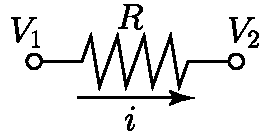
\includegraphics[width=0.5\linewidth]{figures/ohmsLaw}
  
\includegraphics{figures/toDo}
  \caption{This plot shows the power absorbed by the load resistor as its resistance $R_0$ is changed.  The $x$-axis has been normalized by $R_s$, and the $y$-axis has been normalized by the maximum power, $V_s/R_s^2$.}
  \label{fig:maxPower}
\end{figure}
